%&latex
\documentclass[a4paper]{article}

\frenchspacing

\usepackage[cp1250]{inputenc}
\usepackage[czech]{babel}

\usepackage{a4wide}
\usepackage{amsmath, amsthm, amssymb, amsfonts}
\usepackage[mathcal]{eucal}
\usepackage{graphicx}
\usepackage{url}
\usepackage{color}
\usepackage{wrapfig}
\usepackage{capt-of}
\usepackage{float}
\usepackage{ifthen}
\usepackage{subfig}
\usepackage[normalem]{ulem}
\usepackage{pifont}

% sirka a vyska textu nastavena jako papir, vsechny okraje vynulovany a pridano 20pt na kazdou stranu
% horizontalni rozmery
\setlength{\textwidth}{\paperwidth}
\addtolength{\textwidth}{-40pt}
\addtolength{\hoffset}{-1in}
\addtolength{\hoffset}{20pt}
\setlength{\oddsidemargin}{0in}
\setlength{\marginparsep}{0in}
% vertikalni rozmery
\setlength{\textheight}{\paperheight}
\addtolength{\textheight}{-60pt}
\addtolength{\voffset}{-1in}
\addtolength{\voffset}{20pt}
\setlength{\topmargin}{0in}
\setlength{\headheight}{0in}
\setlength{\headsep}{0in}


%Obrazek na miste
%pouziti
%%\obrazeknahore{adresa}{popisek}{label}
\long\def\obrazeknahore#1#2#3 {

\begin{figure}[t]
    \centering
    \includegraphics[width=0.8\textwidth]{#1}
    
    \caption{#2}
    \label{#3}
    
\end{figure}

}


%==========================================
%PEKELNA MAKRA NA ZAROVNANI OBRAZKU DOPRAVA

\makeatletter


%tohle je makro, ktere mi dovoluje obtekani i u kratkych environmentu
%ABSOLUTNE nechapu, jak to funguje, ale funguje to
%viz http://tex.stackexchange.com/questions/26078/ 
\def\odrovnej{\@@par
\ifnum\@@parshape=\z@ \let\WF@pspars\@empty \fi % reset `parshape'
\global\advance\c@WF@wrappedlines-\prevgraf \prevgraf\z@
\ifnum\c@WF@wrappedlines<\tw@ \WF@finale \fi}

\makeatother



%---
%makro, co da obrazek doprava a ostatni text ho obteka
%(bez toho predchazejiciho makra to ale poradne nebeha)
%pouziti:
%\obrazekvpravo{adresa}{popisek}{label}{procento sirky}
\long\def\obrazekvpravo#1#2#3#4{

\setlength\intextsep{-20pt}

    \begin{wrapfigure}{r}{#4\textwidth}
      \begin{center}
          \vspace{-10pt}
          
        \includegraphics[width=#4\textwidth]{#1}
        \vspace{-10pt}
        
      \end{center}
      
      \caption{#2}
      \label{#3}
      
      
    \end{wrapfigure}

\setlength\intextsep{0pt}

    
}




%---
%makro pro pripady, kdy wrapfigure neco mrsi
%je to docela pekelne
%je nutne mu dat jak text vpravo, tak text vlevo
%a nevim, jestli bude 100% fungovat, ale doufam, ze jo

%pouziti:
%\obrazekvpravominipage{adresa}{popisek}{label}{procento sirky}{1 - procento sirky}{text vlevo}
\long\def\obrazekvpravominipage#1#2#3#4#5#6{

\noindent\begin{minipage}{#5\linewidth}
\vspace{0pt}
#6
\end{minipage}
\hspace{0.5cm}
\noindent\begin{minipage}{#4\linewidth}
\vspace{0pt}
\centering
\includegraphics[width=0.9\textwidth]{#1}
\captionof{figure}{#2}
\label{#3}
\end{minipage}

}

%KONEC PEKELNYCH MAKER
%=====================

\def\lebka{
\includegraphics[width=3mm]{../common/lebka}}

% makra pro poznamku u vyrokove a predikatove logiky
\def\vl{ -- ve v�rokov� logice}
\def\pl{ -- v predik�tov� logice}


%Vacsina prostredi je dvojjazicne. V pripade, ze znenie napr pozorovania je pisane po slovensky, malo by byt po slovensky aj oznacenie.

\def\ifis#1#2{\ifthenelse{\equal{#1}{0}}{}{#2}}

%\newenvironment{e}[3]{\pagebreak[2]\noindent\textbf{\ifis{#2}{$\bigstar$}#1}\ifis{#3}{\emph{~(#3)}}\par\noindent\leftskip 10pt }{\odrovnej\par\bigskip}
\newenvironment{e}[3]{\pagebreak[2]\noindent\textbf{\ifis{#2}{\lebka~}#1}\ifis{#3}{\emph{~(#3)}}\ifis{#2}{~\lebka}\par\noindent\leftskip 10pt }{\odrovnej\par\bigskip}


%obecne prostredie, ktore ma vyuzitie pri specialnych odstavcoch ako (uloha, algoritmus...) aby nevzniklo dalsich x prostredi
\newenvironment{obecne}[1]{\pagebreak[2]\noindent\textbf{#1}\par\noindent\leftskip 10pt}{\odrovnej\par\bigskip}

\newenvironment{report}{\pagebreak[2]\noindent\textbf{Report}\em\par\noindent\leftskip 10pt}{\par\bigskip}

%\newenvironment{reportN}[1]{\pagebreak[2]\noindent\textbf{Report~}\emph{(#1)}\emph\par\noindent\leftskip 10pt}{\odrovnej\par\bigskip}
\newenvironment{reportN}[1]{\pagebreak[2]\noindent\textbf{Report~}\emph{(#1)}\em\par\noindent\leftskip 10pt}{\odrovnej\par\bigskip}

\newenvironment{penumerate}{
\begin{enumerate}
  \setlength{\itemsep}{1pt}
  \setlength{\parskip}{0pt}
  \setlength{\parsep}{0pt}
  %\setlength{\topsep}{200pt}
  \setlength{\partopsep}{200pt}
}{\end{enumerate}}

\def\pismenka{\numberedlistdepth=2} %pouzit, ked clovek chce opismenkovany zoznam...

\newenvironment{pitemize}{
\begin{itemize}
  \setlength{\itemsep}{1pt}
  \setlength{\parskip}{0pt}
  \setlength{\parsep}{0pt}
}{\end{itemize}}

\definecolor{gris}{gray}{0.95}
\newcommand{\ramcek}[2]{\begin{center}\fcolorbox{white}{gris}{\parbox{#1}{#2}}\end{center}\par}


\begin{document}

\setcounter{section}{1}
\setcounter{page}{13}
\section{Automaty a jazyky}
\begin{e}{Po�adavky}{0}{0}
\begin{pitemize}
\item Chomsk�ho hierarchie, t��dy automat� a gramatik, determinismus a nedeterminismus.
\item Uz�v�rov� vlastnosti t��d jazyk�.
\end{pitemize}
\end{e}
\input{informatika/teoreticka_informatika/Automaty.O!PS.tex}
\newpage
%&latex
\subsection{Uz�v�rov� vlastnosti t��d jazyk�\footnote{Zdroj tabulky: \url{http://en.wikipedia.org/wiki/Formal_language#Operations_on_languages}}}
\begin{center}

\def\ano{\textcolor{green}{\ding{52}}}
\def\ne{\textcolor{red}{\ding{54}}}

\begin{tabular}{| p{2.4cm} | 1 | 1 | 1 | 1 | 1 | 1 | }
\hline          
    & ~RJ~ & DBKJ & ~BKJ & ~KJ~ & ~RekJ~ & ~RSJ \\          
\hline                         
Sjednocen� & \ano & \ne & \ano & \ano & \ano & \ano  \\
\hline            
  Pr�nik & \ano & \ne & \ne & \ano & \ano & \ano  \\
\hline            
  Pr�nik s RJ & \ano & \ano & \ano & \ano & \ano & \ano  \\
\hline 
  Dopln�k ($-L$) & \ano & \ano & \ne & \ano & \ano & \ne  \\
\hline 
  Homomorfismus / Substituce & \ano & \ne & \ano & \ne & \ne & \ano  \\
\hline 
  Inverzn� homo. & \ano & \ano & \ano & \ano & \ano & \ano \\
\hline
\hline  
  Zrcaden� ($L^R$) & \ano & \ne & \ano & \ano & \ano & \ano  \\
\hline  
  Z�et�zen� & \ano & \ne & \ano & \ano & \ano & \ano  \\
\hline             
  Iterace ($L^*$) & \ano & \ne & \ano & \ano & \ano & \ano  \\
\hline             
  Rozd�l  & \ano & \ne & \ne & \ano & \ano & \ano  \\
\hline  
\end{tabular}
\end{center}
Rozd�l lze vyj�d�it pomoc� pr�niku a dopl�ku tak�e z nich vypl�v�.\\
Pozor KJ nejsou uzav�en� na substituci tak jak ji definuje Bart�k\footnote{viz nap�.:
\url{http://planetmath.org/encyclopedia/RegularSubstitution.html} v tabulce
ve en-wikipedii se mluv� asi o $\lambda$-free substituci}.

\subsubsection*{Bezkontextov� jazyky}

\begin{e}{Pozn�mka}{0}{(D)BKJ nejsou uzav�en� na pr�nik}
sta�� naj�t dva BKJ, jejich� pr�nik nen� BKJ:\\
$L_1 = \{a^ib^ic^j | 0\leq i,j\} \{S\rightarrow AC, A \rightarrow aAb | \lambda, C \rightarrow cC | \lambda\}$\\
$L_2 = \{a^ib^jc^j | 0\leq i,j\} \{S\rightarrow AB, A \rightarrow aA | \lambda, B \rightarrow bBc | \lambda\}$\\
$L_1 \cap L_{2} = \{a^ib^ic^i | 0\leq i\}$ nen� BKJ (v�me z pumping lemmatu)\\
paraleln� b�h dvou z�sobn�kov�ch automat�: ��d�c� jednotky um�me spojit (viz kone�n� automaty), �ten� um�me spojit (jeden automat m��e �ekat), bohu�el dva z�sobn�ky nelze obecn� spojit do jednoho (dva z�sobn�ky = Turing�v stroj, rekurzivn� spo�etn� jazyky)
\end{e}

\begin{e}{Pozn�mka}{0}{(D)BKJ jsou uzav�en� na pr�nik s RJ}
z�sobn�kov� a kone�n� automat m��eme spojit

kone�n� automat $A_1 = (Q_1,X,\delta_1,q_1,F_1)$

z�sobn�kov� automat (p�ij�m�n� stavem) $M_2 = (Q_2,X,Y,\delta_2,q_2,Z_0,F_2)$

nov� automat $M = (Q_1 � Q_2, X, Y, \delta, (q_1,q_2), Z_0, F_1 � F_2)$

~~$((p�,q�), u) \in\delta((p,q),a,Z)$ pr�v� kdy�

~~� $a\neq\lambda: p�\in\delta_1(p,a)\ \&\ (q�,u)\in\delta_2(q,a,Z)$ � automaty �tou vstup

~~� $a=\lambda: (q�,u)\in\delta_2(q,\lambda,Z)$ � ZA m�n� z�sobn�k

~~~~~~~~~~~~~~~$p�=p$ � KA stoj�

z�ejm� $L(M) = L(A_1)\cap L(M_2)$ (paraleln� b�h automat�)
\end{e}

\begin{e}{Pozn�mka}{0}{BKJ jsou uzav�en� na sjednocen�}
pou�ijeme gramatiky (pro ZA nedeterministick� rozeskok na startu)\\
$L_1=L(G_1)$ $G_1 = (V_{N1},V_{T1},S_1,P_1)$\\
$L_2=L(G_2)$ $G_2 = (V_{N2},V_{T2},S_2,P_2)$\\
m��eme p�edpokl�dat, $�e V_{N1} \cap V_{N2} = \varnothing$ (jinak p�ejmenuj)\\
ud�l�me gramatiku:

$G = (V_{N1} \cup V_{N2} \cup \{S\}, V_{T1} \cup V_{T2}, S, P_1 \cup P_2 \cup \{S \rightarrow S_1 | S_2\})$\\
z�ejm� $L(G) = L(G_1) \cup L(G_2)$

�po��t� jedna nebo druh� gramatika
\end{e}

\begin{e}{Pozn�mka}{0}{BKJ nejsou uzav�en� na dopln�k}
sporem podle de Morganov�ch pravidel\\
$L_1 \cap L_2 = -(-L_1 \cup -L_2)$\\
bezkontextov� jazyky nejsou uzav�en� na pr�nik - SPOR\\
v ZA nesta�� prohodit koncov� a nekoncov� stavy!
\end{e}

\begin{e}{Definice}{0}{Substituce a homomorfismus}
\textit{Substituce} $\sigma$ p�ev�d� slova na jazyky

\sigma(\lambda) = \lambda, \sigma(x) = jazyk

\sigma(uv) = \sigma(u). \sigma(v) ~~\sigma: X^* \rightarrow P(Y^*)

\sigma(L) = \cup_{w\in L} \sigma(w)

T��da T jazyk� je uzav�ena na substituci, kdy�: \forall a\in X: \sigma (a)\in
T~\&~ L\in T \Rightarrow \sigma(L)\in T$
\\\\
\textit{Homomorfismus} p�ev�d� slova na slova

$h(\lambda) = \lambda, h(x) = slovo

$h(uv) = h(u) . h(v) ~~h: X^* \rightarrow Y^*

$h(L) = \{h(w) | w\in L\}$
\\\\
\textit{Inverzn� homomorfismus} p�ev�d� slova zp�t
h^{-1}(L) = \{ w | h(w)\in L\}
\end{e}

\begin{e}{Pozn�mka}{0}{BKJ jsou uzav�eny na substituci}
intuitivn�: listy v deriva�n�m stromu generuj� dal�� stromy
\\
form�ln�:
m�me bezkontextov� jazyk $L_0$, tj. gramatiku $G_0 = (V_{N0},V_{T0},S_0,P_0)$,
pro ka�d� termin�l ai z  $V_{T0}$, $\sigma(a_i)$ je bezkontextov� jazyk - gramatika $G_i$ p�edpokl�dejme, �e mno�iny netermin�l� jsou navz�jem disjunktn�
a �e ��dn� termin�l nen� v jin� gramatice netermin�lem

definujme $G = (\cup_{i\geq0}V_{Ni}, \cup_{i\geq1}V_{Ti}, S_0, P)$, kde

$P = \cup_{i\geq1}P_i \cup P'$ a $P' = P_0$, kde ka�d� termin�l $a_i$ je nahrazen $S_i$

z�ejm�: $L(G) = \sigma(L_0)$
\\
P��klad:

\begin{minipage}{0.2\linewidth}
$L_0 = \{a^ib^j ~|~ 0\leq i\leq j\}$ \\
$\sigma(a) = L_1 = {c^id^i | 0\leq i\}$ \\
$\sigma(b) = L_2 = {c^i | 0\leq i\}$ \\
$\sigma(L_0):$
\end{minipage}
\noindent\begin{minipage}{0.4\linewidth}
\vspace{0.3cm}
$S_0 \rightarrow aS_0b | S_0b | \lambda$ \\
$S1 \rightarrow cS_1d | \lambda$ \\
$S2 \rightarrow cS_2 | \lambda$ \\
$S0 \rightarrow S_1S_0S_2 | S_0S_2 | \lambda,~ S_1 \rightarrow cS_1d | \lambda,~ S_2 \rightarrow cS_2 | ?$ \\
\end{minipage}
\noindent\begin{minipage}{0.1\linewidth}
\vspace{0pt}
\centering
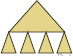
\includegraphics[width=0.9\textwidth]{informatika/teoreticka_informatika/obrazky/der_strom.png}
\end{minipage}

\end{e}

\begin{e}{Pozn�mka}{0}{BKJ jsou uzav�eny na homomorfismus}
p��m� d�sledek p�edchoz� v�ty (termin�l nahrad�me slovem)
\end{e}

\begin{e}{Pozn�mka}{0}{BKJ jsou uzav�eny na inverzn� homomorfismus}
$h^{-1}(L) = \{ w | h(w)\in L\}$ - m�me z�sobn�kov� automat M pro L a �teme w\\
idea:

� p�e�teme p�smeno x a do vnit�n�ho bufferu d�me h(x)

� simulujeme v�po�et M, kdy vstup bereme z bufferu

� po vypr�zdn�n� bufferu na�teme dal�� p�smeno ze vstupu

� slovo je p�ijato, kdy� je buffer pr�zdn� a M je v koncov�m stavu
\\
form�ln�:

buffer je kone�n�, m��eme ho tedy modelovat ve stavu
pro $L$ m�me $M = (Q,X,Y,\delta,q_0,Z_0,F)$ (p��j�m�n� koncov�m stavem)

$h: A^* \rightarrow X^*$

definujme $M' = (Q', A, Y, \delta',[q_0,\lambda], Z_0, F�\{\lambda\})$, kde

$Q' = \{[q,u] ~|~ q\in Q,~ u\in X^*, ~\exists a\in A ~\exists v\in X^* ~h(a)=vu\}$, u je buffer

$\delta'([q,u], \lambda, Z) = \{ ([p,u],\gamma) | (p,\gamma) \in \delta(q, \lambda, Z) \}$

~~~~~~~~~~~~~~~~~~$\cup~ \{ ([p,v],\gamma ) ~|~ (p,\gamma) \in (q, b, Z) \}$ � $u=bv$ (�te buffer)

$\delta'([q, \lambda], a, Z) = \{ ([q,h(a)],Z) \}$ � napl�uje buffer
\end{e}

\begin{e}{Pozn�mka}{0}{DBKJ nejsou uzav�en� na sjednocen� (BKJ ano)!}
P��klad:

$L = {a^ib^jc^k ~|~ i\neq j ~OR~ j\neq k ~OR~ i\neq k\}$ je BKJ, ale nen� DBKJ

sporem: nech� $L$ je DBKJ
potom $-L$ (dopln�k) je DBKJ

$-L \cap a*b*c* = \{a^ib^jc^k | i=j=k\}$ je DBKJ - SPOR
\end{e}

\begin{e}{Pozn�mka}{0}{DBKJ nejsou uzav�en� na homomorfismus (BKJ ano)!}
P��klad:

$L_1 = \{a^ib^jc^k | i=j\}$ je DBKJ

$L_2 = \{a^ib^jc^k | j=k\}$ je DBKJ

$0L_1 \cup 1L_2$ je DBKJ, $1L_1 \cup 1L_2$ nen� DBKJ

polo�me $h(0) = 1$ a $h(x) = x$ pro ostatn� symboly

$h(0L_1 \cup 1L_2) = 1L_1 \cup 1L_2$
\end{e}



\begin{e}{Pozn�mka}{0}{Dopln�k deterministick�ho BKJ je op�t deterministick� BKJ!}
prohod�me koncov� a nekoncov� stavy\\
pot�e:\\
� nemus� p�e��st cel� vstupn� slovo\\
� krok nen� definov�n (nap�. vypr�zdn�n� z�sobn�ku)

snadno o�et��me �podlo�kou� na z�sobn�ku\\
� cyklus (z�sobn�k roste, z�sobn�k pulsuje)

odhal�me pomoc� ��ta�e\\
� po p�e�ten� slova proch�z� koncov� a nekoncov� stavy

sta�� si pamatovat, zda pro�el koncov�m stavem
\end{e}

\subsubsection*{Kontextov� jazyky}

\begin{e}{Pozn�mka\footnote{J.Hopcroft,J.Ullmann: FORMAL LANGUAGES AND THEIR RELATION TO AUTOMATA, str.127}}{0}{KJ nejsou uzav�en� na substituci a homomorfismus}
Proof Let $G_1 = (V_N, V_T, P_1, S)$ be a type 0 grammar such that $L(G_1)$ is
not a context-sensitive language. We assume without loss of
generality that the productions are of the form $\alpha\rightarrow\beta$ or $A\rightarrow a$, where $\alpha\in V^+_N$, $\beta \in V^*_N$, $A \in V_N$, and $a \in V_T$. Let $c$ be a new symbol.
\\Consider the grammar $G_2 = (V_N, V_T\cup \{C\}, P_2, S)$ where $P_2$ contains:
\\1. $\alpha\rightarrow\beta$ if $\alpha\rightarrow\beta$ is in $P_2$ and $|\alpha|\leq|\beta|$.
\\2. $\alpha\rightarrow\beta cc...c$ where $|\alpha|=|\beta cc...c|$ if $\alpha\rightarrow\beta$ is in $P_2$ and $|\alpha|<|\beta|$.
\\3. $cA\rightarrow Ac$ $\forall A \in V_N$.
\\The grammar $G_2$ is context sensitive, since we have forced the right-hand
side of every Production to be at least as long as the left-hand side. The
productions $cA\rightarrow Ac$ were added to move the $c$'s to the right end of
the words so that derivations in $G_2$ can proceed as in $G_1$. Now consider the
substitution
\\$\sigma(a) = \{a\}$ for $a \in V_T$ and $\sigma(c) = \{\lambda\}$.
\\Then $\sigma(L(G_2)) = L(G_1)$ (a type 0 grammar) and hence substitution does not preserve the class
of Context-sensitive languages.
\\\\ \LARGE\sun\normalsize~ The substitution used in the proof is a homomorphism.
\end{e}

\subsubsection*{Rekurzivn� a rekurzivn� spo�etn� jazyky}

\begin{e}{V�ta}{0}{Postova}
$L$ je rekurzivn� $\Leftrightarrow$ $-L$ a $L$ jsou rekurzivn� spo�etn�
\end{e}

\begin{e}{Pozn�mka\footnote{Zdroj: \url{http://youbo2010.blogspot.com/2011/04/why-recursive-languages-are-not-closed.html}}}{0}{RSJ
jsou a RekJ nejsou uzav�en� na homomorfismus}
First let's consider a much simpler problem, inverse homomorphism, in which w is in L' if and only h(w) is in L. We can just apply h to w and let the TM accepting L run with input h(w). So L' is recursively enumerable(resp. recursive) if L is recursively enumerable(resp. recursive).
\\\\
Now we'll attack homomorphism, in which $x\in L' \Leftrightarrow \exists
w\in L : h(w)=x$.
\\\\
For recursively enumerable languages, the slide say that we can design an NTM M to take as input $x$, guess an $w$ such that $h(w)=x$ and simulate $M_1$ on $w$ (suppose $L=L(M_1)$). I will give a detailed sketch on how $M$ behaves. It

0) sets $l$ to 1

1) guesses one $w$ of length $l$

2) if there is such an $w$ invokes $M_1$ otherwise goes to 4)

3) if $M_1$ accepts so would M otherwise goes to 4)

4) increases $l$ by 1 and goes back to 1)
\\\\
So if $L$ is recursively enumerable, so is $L'$.
And of course we can use a DTM that generates each $w$ in a systematic way.
\\\\
Now what about recursive languages? Even though $L$ is recursive, the above process may not halt since there may be infinitely many $w$'s such that $h(w)=x$ but none of these $w$'s is in $L$. A automat $M$ se prost� zacykl�.
\\\\
To show recursive languages not closed under homomorphism, consider
the language $L=\{<M,w, a^i> |$ TM M accepts w in i steps$\}$, which is recursive.
However, if a homomorphism h maps a to $\lambda$ while keeping the remaining symbols intact, $h(L)=\{<M,w> |$ TM M accepts w$\}$ which is not recursive.\footnote{http://www.cs.uiuc.edu/class/fa10/cs373/lectures/lect18.pdf}
\end{e}

\begin{e}{Pozn�mka}{0}{Dopln�k RekJ mus� v�dy b�t RekJ}
Nech� jazyk L je rekurzivn�. Pak jist� existuje TS M, kter� tento jazyk rozhoduje. Tento TS M pracuje tak, �e v�echna slova w z L p�ijme a v�echna slova z -L (= dopln�k jazyka L) odm�tne. Nov� TS M', kter� bude rozhodovat jazyk -L sestroj�me takto:

    $\bullet$ Simuluj �innost TS M pro vstup w.

    $\bullet$ Pokud TS M slovo p�ijme, odm�tni. Pokud TS M slovo odm�tne, p�ijmi.
\\
Nov� TS M' bude jednodu�e vracet p�esn� opa�n� v�sledky, ne� p�vodn� TS M. Tento TS M' rozhoduje jazyk -L.
\end{e}

\begin{e}{Pozn�mka}{0}{Dopln�k RSJ nemus� v�dy b�t RSJ}
Komplementem �ist� RSJ (tedy jazyka, kter� je RSJ, ale nen� rekurzivn�) je v�dy jazyk, kter� nen� rekurzivn� spo�etn�. Vezm�me pro p��klad jazyk HALT, kter� je �ist� RSJ, ale jeho komplement (NotHALT) nen� RSJ. To vypl�v� z definice NotHALT: HALT obsahuje dvojice TS:slovo takov�, �e TS pro dan� slovo zastav�. NotHALT tedy obsahuje dvojice TS:slovo takov�, kdy dan� TS nezastav� pro slovo, �e se zacykl�. Proto�e nejsme schopni identifikovat cyklus, nejsme schopni sestavit TS, kter� by jazyk NotHALT p�ij�mal. Obecn�: pokud m�me jazyk L, kter� je �ist� RSJ, pak jeho komplement -L mus� obsahovat takov� slovo, pro n� se TS M' zacykl� a tud� tento TS M' nem��e p�ij�mat jazyk -L.
\end{e}

TODO: nejaka zduvodneni chyb�



\end{document}
